\begin{name}
	{\tenchude}
	{ĐỀ KSCL - THPT ĐỒNG HỶ - THÁI NGUYÊN}
	{LỚP TOÁN THẦY PHÁT}
	{\lq\lq  Nothing will work unless you do.\rq\rq}
\end{name}

\Opensolutionfile{ansbook}[ans/ansb\currfilebase]
\caulc
\Opensolutionfile{ans}[ans/ans\currfilebase-Phan-I]
\begin{ex}%[Nguyễn Tuấn, dự án đề thi thử các trường, Sở lần 1 năm 2026]%[2H2H1-2]%Câu 1
	Cho hình chóp $S.ABCD$ có đáy $ABCD$ là hình bình hành. Gọi $O$ là tâm của hình bình hành $ABCD$. Mệnh đề nào sau đây đúng? 
	\choice
	{$\overrightarrow{SA}+\overrightarrow{SB}+\overrightarrow{SC}+\overrightarrow{SD}=\overrightarrow{SO}$}
	{$\overrightarrow{SA}+\overrightarrow{SB}+\overrightarrow{SC}+\overrightarrow{SD}=2\overrightarrow{SO}$}
	{\True $\overrightarrow{SA}+\overrightarrow{SB}+\overrightarrow{SC}+\overrightarrow{SD}=4\overrightarrow{SO}$}
	{$\overrightarrow{SA}+\overrightarrow{SB}+\overrightarrow{SC}+\overrightarrow{SD}=\overrightarrow{0}$}
	\loigiai{
\immini{
Trong tam giác $SAC$ ta có $\overrightarrow{SA}+\overrightarrow{SC}=2\overrightarrow{SO}$ .\\
Trong tam giác $SBD$ ta có $\overrightarrow{SB}+\overrightarrow{SD}=2\overrightarrow{SO}$ .\\
Vậy $\overrightarrow{SA}+\overrightarrow{SB}+\overrightarrow{SC}+\overrightarrow{SD}=4\overrightarrow{SO}$.
	}{
\begin{tikzpicture}[scale=0.7, font=\footnotesize, line join=round, line cap=round, >=stealth]
	\path 
	(0,0)coordinate(A)++(0:4)coordinate(D)++(210:2)coordinate(C)++(180:4)coordinate(B)
	(A)++(80:3)coordinate(S)
	($(A)!.5!(C)$)coordinate(O)
	;
	\draw 
	(S)--(B)--(C)--(D)--(S)--(C)
	;
	\draw [dashed] 
	(B)--(A)--(D)--(B) (C)--(A)--(S)--(O)
	;
	\foreach \i/\g in {S/90,A/-90,B/-90,C/-90,D/0,O/-90}{\draw[fill=black](\i) circle (1pt) ($(\i)+(\g:3mm)$) node[scale=1]{$\i$};}
\end{tikzpicture}	
}}
\end{ex}
\begin{ex}%[Nguyễn Tuấn, dự án đề thi thử các trường, Sở lần 1 năm 2026]%[2D1N4-1]
	Cho hàm số $y=\dfrac{x+2\,026}{x-2\,025}$ có đồ thị $(C)$. Đồ thị $(C)$ có đường tiệm cận đứng là
	\choice
	{\True $x=2\,025$}
	{$x=-2\,024$}
	{$x=1$}
	{$x=6$}
	\loigiai{
		Tập xác định $\mathscr{D}=\mathbb{R}\setminus \{2\,025\}$.\\
		Ta có
		$$\lim\limits_{x\to2\,025^+}\dfrac{x+2\,026}{x-2\,025}=+\infty.$$
		Do đó đồ thị $(C)$ có đường tiệm cận đứng là $x=2\,025$.}
\end{ex}

\begin{ex}%[Nguyễn Tuấn, dự án đề thi thử các trường, Sở lần 1 năm 2026]%[2D1H3-1]%Câu 3
	Giá trị lớn nhất của hàm số $y=x^3-3x+1$ trên đoạn $[-2;2]$ là
	\choice
	{$ 2$}
	{$-1$}
	{\True $3$}
	{$-2$}
	\loigiai{
		Ta có $y=x^3-3x+1$.\\
		Tập xác định $\mathscr{D}=\mathbb{R}$.\\
		Ta có, $y'=3x^2-3$, $y'=0\Leftrightarrow\hoac{&
			x=1\\&
			x=-1.}$\\
		Ta có $y(-2)=-1$, $y(2)=3$, $y(-1)=3$, $y(1)=-1$.\\
		Vậy giá trị lớn nhất của hàm số $y=x^3-3x+1$ trên đoạn $[-2;2]$ là $3$.}
\end{ex}

\begin{ex}%[Nguyễn Tuấn, dự án đề thi thử các trường, Sở lần 1 năm 2026]%[2D3H1-3]%Câu 4
	Cho bảng số liệu khảo sát về tuổi thọ (đơn vị: nghìn giờ) của một loại bóng đèn:
\begin{center}
\begin{tabular}{|c|c|c|c|c|c|}
	\hline Tuổi thọ & {$[3;5)$} &{$[5;7)$}&{$[7;9)$}&{$[9;11)$} & {$[11;13)$} \\
	\hline Số bóng đèn & $11$ & $20$ & $29$ & $40$ & $30$ \\
	\hline
\end{tabular}
\end{center}
	Giá trị của tứ phân vị thứ nhất là
	\choice
	{\True $Q_1=\dfrac{206}{29}$}
	{$Q_1=\dfrac{37}{4}$}
	{$Q_1=\dfrac{87}{8}$}
	{$Q_1=\dfrac{875}{232}$}
	\loigiai{
		Ta có cỡ mẫu là $n=130$ và
		$\dfrac{n}{4}=32{,}5$ .\\
		Nhóm $[7;9)$ là nhóm đầu tiên có tần số tích luỹ lớn hơn hoặc bằng $32{,}5$.\\
		Vậy $Q_1=7+\dfrac{32{,}5-(20+11)}{29}\cdot (9-7)=\dfrac{206}{29}$.}
\end{ex}

\begin{ex}%[Nguyễn Tuấn, dự án đề thi thử các trường, Sở lần 1 năm 2026]%[1H8H6-1]%Câu 5
\immini
{
		Cho hình hộp chữ nhật $ABCD.A'B'C'D'$ có $AB=BC=a$, $AA'=a\sqrt{2}$ (như hình vẽ). Góc giữa đường thẳng $A'C$ và mặt phẳng $(ABCD)$ bằng
\choice{$60^\circ$}{\True $45^\circ$}{$30^\circ$}{$90^\circ$}
}
{
\begin{tikzpicture}[>=stealth,line join=round,line cap=round,font=\footnotesize,scale=1]
	\path (0,0)coordinate(A)
	(-150:1.5)coordinate(B)
	(2,0)coordinate(D)
	($(B)+(D)-(A)$)coordinate(C)
	($(A)+(0,2)$)coordinate(A')
	($(A')+(C)-(A)$)coordinate(C')
	($(A')+(B)-(A)$)coordinate(B')
	($(A')+(D)-(A)$)coordinate(D')
	
	;
	\draw(A')--(B')--(B)--(C)--(D)--(D')--cycle
	(B')--(C')--(D')
	(C)--(C')
	;
	\draw[dashed](B)--(A)--(D)
	(A)--(A')--(C)
	(A)--(C)
	;
	\foreach \x/\g in {A/-90,B/-90,C/-90,D/0,A'/90,B'/90,C'/60,D'/90}\fill[black](\x)circle(1pt)+(\g:.3)node{$\x$};
\end{tikzpicture}
}
	\loigiai{
		Ta có góc giữa đường thẳng $A'C$ và mặt phẳng $(ABCD)$ bằng góc giữa $A'C$ và $AC$.\\
		Xét tam giác $ AA'C$ vuông tại $A$ ta có $\tan\widehat{A'AC}=\dfrac{A'A}{AC}=1\Rightarrow\widehat{A'AC}=45^\circ$.
	}
\end{ex}

\begin{ex}%[Nguyễn Tuấn, dự án đề thi thử các trường, Sở lần 1 năm 2026]%[2H2H1-3]%Câu 6
	Cho hình lập phương $ ABCD.A'B'C'D'$ có $AB=4$. Tính $\left|\overrightarrow{AB}+\overrightarrow{B'C'}+\overrightarrow{AA'}\right|$.
	\choice
{$4\sqrt{2}$}{$\sqrt{10}$}{\True $4\sqrt{3}$}{$2\sqrt{10}$}
	\loigiai{
\immini{
Ta có $\left|\overrightarrow{AB}+\overrightarrow{B'C'}+\overrightarrow{AA'}\right|=\left|\overrightarrow{AB}+\overrightarrow{AD}+\overrightarrow{AA'}\right|=\left|\overrightarrow{AC'}\right|=AC=4\sqrt{3}$.
	}{
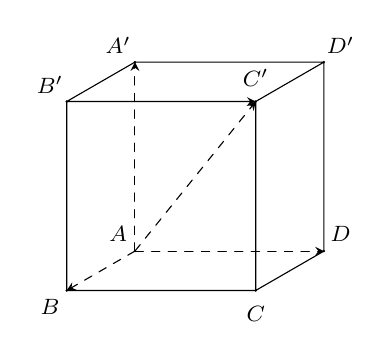
\begin{tikzpicture}[>=stealth,line join=round,line cap=round,font=\footnotesize,scale=0.4]
	\def\r{-150}
	\def\c{6}
	\def\d{2.5}
	\path
	(0:0) coordinate (A)++(0:\c)
	coordinate (D)++(90:\c)coordinate(D')
	(A)++(\r:\d) coordinate (B)++(0:\c) coordinate (C)++(90:\c)coordinate(C')
	(A)++(90:\c) coordinate (A')++(\r:\d) coordinate (B')
	;
	\draw (A')--(B')--(B)--(C)--(D)--(D')--(A') (C)--(C') (B')--(C')--(D');
	%				\draw[dashed] (A')--(A)--(B) (A)--(D);
	\foreach \p / \r in {A/135,B/-135,D/45,A'/135,B'/135,D'/45,C/-90,C'/90}
	\fill (\p) circle (1.2pt) node[shift={(\r:3mm)}]{$\p$};
	\foreach \p / \r in {A/B,A/A',B'/C',A/D,A/C'}
	\draw[->,dashed] (\p)--(\r);
\end{tikzpicture}	
}}
\end{ex}

\begin{ex}%[Nguyễn Tuấn, dự án đề thi thử các trường, Sở lần 1 năm 2026]%[2D1N2-2]%Câu 7
	Cho hàm số $ y=f(x)$ có bảng biến thiên như sau
\begin{center}
	
\begin{tikzpicture}
		\tkzTabInit[lgt=1.2,espcl=3]
		{$x$/0.8, $f’(x)$/0.8, $f(x)$/2.5}
		{$-\infty$,$2$,$3$,$+\infty$}
		\tkzTabLine{ ,-,0,+,0,-, }
		\tkzTabVar{+/$+\infty$,-/$-1$,+/$2$,-/$-\infty$}
	\end{tikzpicture}
\end{center}
	Điểm cực đại của hàm số $ y=f(x)$ là
	\choice
	{$y=2$}{$x=2$}{\True $x=3$}{$y=-1$}
	\loigiai{
		Điểm cực đại của hàm số $y=f(x)$ là $x=3$.
	}
\end{ex}

\begin{ex}%[Nguyễn Tuấn, dự án đề thi thử các trường, Sở lần 1 năm 2026]%[1D6H4-3]%Câu 8
	Tập nghiệm của bất phương trình $\left(\dfrac{1}{2}\right)^{x^2+4x}>\dfrac{1}{32}$ là
	\choice
	{\True $(-5;1)$}
	{$(1;+\infty)$}
	{$(-\infty ;-5)\cup (1;+\infty)$}
	{\True $\{-5;1\}$}
	\loigiai{
		Ta có $\left(\dfrac{1}{2}\right)^{x^2+4x}>\dfrac{1}{32}\Leftrightarrow\left(\dfrac{1}{2}\right)^{x^2+4x}>\left(\dfrac{1}{2}\right)^5\Leftrightarrow{x^2}+4x < 5\Leftrightarrow-5<x<1$.
	}
\end{ex}

\begin{ex}%[Nguyễn Tuấn, dự án đề thi thử các trường, Sở lần 1 năm 2026]%[1D2H3-4]%Câu 9
	Cho cấp số nhân $(u_n)$ với $u_1=2$ và công bội $q=3$. Tìm số hạng thứ ba $u_3$ của cấp số nhân.
	\choice
	{$6$}
	{$24$}
	{$54$}
	{\True $18$}
	\loigiai{
		Số hạng thứ ba của cấp số nhân là $u_3=u_1\cdot q^2=2\cdot 3^2=18$.}
\end{ex}

\begin{ex}%[Nguyễn Tuấn, dự án đề thi thử các trường, Sở lần 1 năm 2026]%[2H2H1-2]%Câu 10
\immini
[thm]{Cho hình hộp $ ABCD.A'B'C'D'$ (minh họa như hình bên). Phát biểu nào sau đây là {\bf sai}?
	\choice
	{$\overrightarrow{AB}+\overrightarrow{AD}=\overrightarrow{A'C'}$}
	{$\overrightarrow{AA'}+\overrightarrow{AC}=\overrightarrow{AC'}$}
	{$\overrightarrow{BB'}+\overrightarrow{BA}+\overrightarrow{BC}=\overrightarrow{BD'}$}
	{\True $\overrightarrow{DA}+\overrightarrow{DC}=\overrightarrow{B'D'}$}
}
{
\begin{tikzpicture}[line join=round, line cap=round, font=\footnotesize, scale=0.6]
	\coordinate (B) at (0,0);
	\coordinate (A) at (1,.8);
	\coordinate (C) at (4,0);
	\coordinate (D) at ($(C)-(B)+(A)$);
	\coordinate (A1) at ($(A)+(70:4)$);
	\coordinate (B1) at ($(B)-(A)+(A1)$);
	\coordinate (C1) at ($(C)-(A)+(A1)$);
	\coordinate (D1) at ($(D)-(A)+(A1)$);
	
	% Giữ nguyên các nét vẽ của bạn
	\draw (B1)--(B)--(C)--(D)--(D1)--(A1)--(B1)--(C1)--(D1) (C)--(C1);
	\draw[dashed] (A)--(D) (A1)--(A)--(B);
	
	% Chuẩn hóa hiển thị tên điểm A', B', C', D' theo quy tắc của bạn
	\foreach \x/\y/\g in {A/A/180, B/B/-90, C/C/-90, D/D/0, A1/A'/90, B1/B'/180, C1/C'/90, D1/D'/90} 
	\fill[black] (\x) circle (1pt)+(\g:.3) node {$\y$};
\end{tikzpicture}
}
	\loigiai{
		Ta có
\begin{itemize}
	\item $\overrightarrow{AB}+\overrightarrow{AD}=\overrightarrow{AC}=\overrightarrow{A'C'}$.
	\item $\overrightarrow{AA'}+\overrightarrow{AC}=\overrightarrow{AC'}$.
	\item $\overrightarrow{BB'}+\overrightarrow{BA}+\overrightarrow{BC}=\overrightarrow{BD'}$.
	\item $\overrightarrow{DA}+\overrightarrow{DC}=\overrightarrow{DB}=\overrightarrow{D'B'}$.
\end{itemize}
}
\end{ex}
\begin{ex}%[Nguyễn Tuấn, dự án đề thi thử các trường, Sở lần 1 năm 2026]%[2D1H5-1]
	\immini[thm]{Hàm số nào sau đây có đồ thị là đường cong như hình bên?
		\choice
		{$y=x-\dfrac{1}{x-1}$}
		{$y=-x+\dfrac{1}{x-1}$}
		{$y=-x-\dfrac{1}{x-1}$}
		{\True $y=x+\dfrac{1}{x-1}$}}
	{
		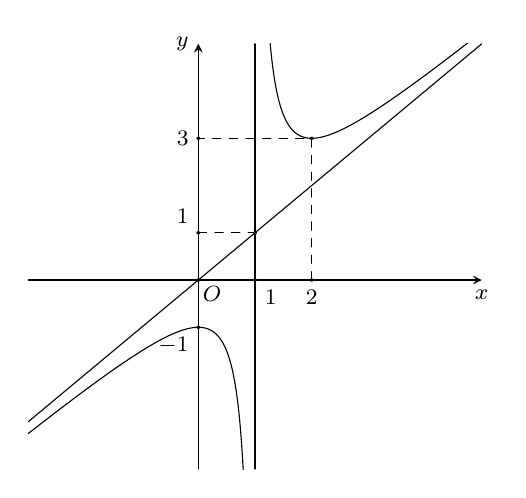
\begin{tikzpicture}[xscale=1.2,scale=0.6, font=\footnotesize, line join=round, line cap=round, >=stealth]
			\def\f(#1){(#1)+(1)/((#1)-1)}
			\def\xmin{-3}
			\def\xmax{5}
			\def\ymin{-4}
			\def\ymax{5}
			\draw[->] (\xmin,0)--(\xmax,0) node[below] { $x$};
			\draw[->] (0,\ymin)--(0,\ymax) node[left] { $y$};
			\fill (0,0) circle(1pt) node[shift=(-45:0.25)]{$O$}
			(1,1) circle (1pt);
			\foreach \x/\a in {1/below right,2/below} \fill (\x,0) circle (1pt) node [\a] { $\x$};
			\foreach \y/\a in {-1/below left,1/above left,3/left} \fill (0,\y) circle (1pt) node [\a] { $\y$};
			\clip (\xmin,\ymin) rectangle (\xmax,\ymax);
			\draw (1,\ymin)--(1,\ymax);
			\draw[smooth,samples=200] plot[domain=\xmin:0.8] (\x,{\f(\x)});
			\draw[smooth,samples=200] plot[domain=\xmin:\xmax] (\x,\x);
			\draw[smooth,samples=200] plot[domain=1.2:\xmax] (\x,{\f(\x)});
			\draw[dashed] (2,0)--(2,3)--(0,3) (0,1)--(1,1);
			\fill (2,3) circle (1pt);
		\end{tikzpicture}
	}
	\loigiai{
		Ta có điểm $(2;3)$ thuộc đồ thị hàm số.\\
		Lần lượt thay $x=2$, $y=3$ vào các phương án, ta có điểm $(2;3)$ chỉ thuộc đồ thị hàm số $y=x+\dfrac{1}{x-1}$.
	}
\end{ex}

\begin{ex}%[Nguyễn Tuấn, dự án đề thi thử các trường, Sở lần 1 năm 2026]%[2H2N2-2]%Câu 12
	Trong không gian $Oxyz$, cho hai điểm $ A(4;-2;2)$ và $B(5;-1;4)$. Tọa độ trọng tâm $G$ của tam giác $OAB$ là
	\choice
	{$ G\left(\dfrac{9}{2};-\dfrac{3}{2};3\right)$}
	{\True $G(3;-1;2)$}
	{$ G(1;1;2)$}
	{$ G(9;-3;6)$}
	\loigiai{
		Tọa độ trọng tâm $ G$ của tam giác $OAB$ là $\heva{&
			{x_G}=\dfrac{4+5}{3}=3\\&
			{y_G}=\dfrac{-2-1}{3}=-1\\&
			{z_G}=\dfrac{2+4}{3}=2} \Rightarrow G(3;-1;2)$.}
\end{ex}
\Closesolutionfile{ans}
\cauds
\Opensolutionfile{ans}[ans/ans\currfilebase-Phan-II]

\begin{ex}%[Nguyễn Tuấn, dự án đề thi thử các trường, Sở lần 1 năm 2026]%[2D1H3-1]%Câu 13
	Cho hàm số $f(x)=-\sin x-\dfrac{1}{2}x$
\choiceTF
{$f(2\pi)=\pi $}
{\True Đạo hàm của hàm số đã cho là $f'(x)=-\cos x-\dfrac{1}{2}$}
{Phương trình $ f'(x)=0$ có $2$ nghiệm phân biệt trên đoạn $[0;\pi]$}
{Giá trị nhỏ nhất của hàm số $f(x)$ trên đoạn $[0;\pi]$ là $-\dfrac{\pi}{2}$}
\loigiai{
\begin{itemchoice}
	\itemch Ta có $f(2\pi)=-\sin 2\pi-\dfrac{1}{2}\cdot 2\pi=-\pi$.
	\itemch Ta có $f'(x)=-\cos x-\dfrac{1}{2}$.
	\itemch Ta có
	$f'(x)=0 \Leftrightarrow-\cos x-\dfrac{1}{2}=0 \Leftrightarrow \cos x=-\dfrac{1}{2} \Leftrightarrow\hoac{&
		x=\dfrac{2\pi}{3}+k2\pi \\&
		x=-\dfrac{2\pi}{3}+m2\pi}\quad (k, m \in \mathbb{Z}).$\\
	Do $x\in[0;\pi]$ nên ta có $k=0$.\\ 
	Phương trình chỉ có $1$ nghiệm thuộc đoạn $[0;\pi]$.
	\itemch Trên đoạn $[0;\pi]$ thì $ f'(x)=0\Leftrightarrow 2\cos x+1=0\Leftrightarrow\cos x=-\dfrac{1}{2}\Leftrightarrow x=\dfrac{2\pi}{3}$.\\
	Ta có $f(0)=0$; $f(\pi)=-\dfrac{\pi}{2}$; $f\left(\dfrac{2\pi}{3}\right)=-\sin\dfrac{2\pi}{3}-\dfrac{1}{2}\cdot\dfrac{2\pi}{3}=-\dfrac{\sqrt{3}}{2}-\dfrac{\pi}{3}$.\\
	Suy ra giá trị nhỏ nhất của hàm số $ f(x)$ trên đoạn $[0;\pi]$ là $-\dfrac{\sqrt{3}}{2}-\dfrac{\pi}{3}$.
\end{itemchoice}
}
\end{ex}

\begin{ex}%[Nguyễn Tuấn, dự án đề thi thử các trường, Sở lần 1 năm 2026]%[2D1H5-1]%Câu 14
\immini
{
Đồ thị cùa hàm số $y=ax+b+\dfrac{c}{x+d}$ là hình bên
\choiceTF
{\True Hàm số nghịch biến trên khoảng $(0;1)$}
{$\lim\limits_{x\to 1^+}y=-\infty $}
{\True Phương trình đường tiệm cận xiên của đồ thị hàm số là $y=x+1$}
{\True Tổng $a+b+c+d=2$}
}
{
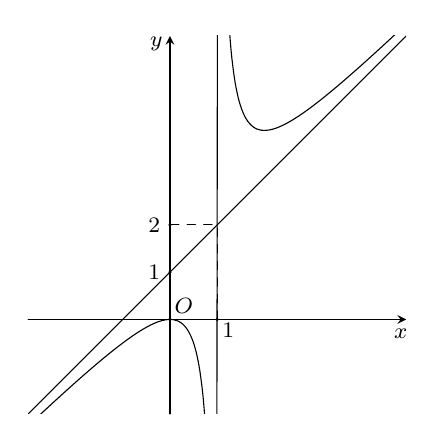
\begin{tikzpicture}[scale=0.6, font=\footnotesize, line join=round,line cap=round, >=stealth]
\def \xmin{-3}
\def \xmax{5}
\def \ymin{-2}
\def \ymax{6}
\draw[->] (\xmin,0)--(\xmax,0) node[shift=(-110:0.2)] {$x$};
\draw[->] (0,\ymin)--(0,\ymax) node[shift=(-150:0.2)] {$y$};
\fill (0,0) circle(1pt) node[shift=(45:0.25)]{$O$}
(1,0) circle(1pt) node[shift=(-45:0.2)]{$1$}
(0,2) circle(1pt) node[shift=(180:0.2)]{$2$}
(0,1) circle(1pt) node[shift=(180:0.2)]{$1$};
\draw[dashed] (1,0)|-(0,2);
\clip (\xmin,\ymin) rectangle (\xmax,\ymax);
\draw[smooth,samples=100,domain=\xmin:\xmax] plot(\x,{(\x)^2/((\x)-1)});
\draw [smooth,samples=100,domain=\xmin:\xmax] plot(\x,{(\x)+1});
\end{tikzpicture}
}
\loigiai{
\begin{itemchoice}
	\itemch Dựa vào đồ thị hàm số, ta thấy hàm số nghịch biến trên khoảng $ (0;1)$.
	\itemch Dựa vào đồ thị hàm số, ta thấy $\lim\limits_{x\to 1^+}y=+\infty$.
	\itemch Phương trình đường tiệm cận xiên của đồ thị hàm số có dạng $ y=ax+b$.\quad (1)\\
	Do đường tiệm cận xiên đi qua $2$ điểm $(0;1)$ và $(1;2)$, ta thay vào $(1)$ ta có hệ phương trình:
	$\heva{&
		b=1\\&
		a+b=2} \Leftrightarrow\heva{&
		b=1\\&
		a=1} \Rightarrow $ phương trình đường tiệm cận xiên của đồ thị hàm số là $y=x+1$.
	\itemch Dựa vào đồ thị hàm số, phương trình đường tiệm cận đứng là $x=1$.\\
	Nên mẫu số có dạng $x-1\Rightarrow d=-1$.\\
	Kết hợp phương trình đường tiệm cận xiên của đồ thị hàm số là $ y=x+1$.\\
	Ta có $y=x+1+\dfrac{c}{x-1}$.\quad (2)\\
	Đồ thị hàm số đi qua điểm $(0;0)$ thay vào $(2)$ ta được $ 0+1+\dfrac{c}{0-1}=0\Leftrightarrow c=1$.\\
	Vậy tổng $ a+b+c+d=1+1+1-1=2$.
\end{itemchoice}
}
\end{ex}

\begin{ex}%[Nguyễn Tuấn, dự án đề thi thử các trường, Sở lần 1 năm 2026]%[2H2V2-6]%Câu 15
Trong không gian $ Oxyz$ có $\overrightarrow{i}$, $\overrightarrow{j} $, $\overrightarrow{k}$ lần lượt là các vectơ đơn vị trên các trục $Ox$, $Oy$, $Oz$. Cho hai điểm $A$ và $B$. Biết $A$ có hình chiếu vuông góc lên mặt phẳng $(Oxy)$ là một điểm thuộc tia $Ox$. Góc hợp bởi $OA$ và mặt phẳng $(Oxy)$ là $\alpha$ với $\sin\alpha=\dfrac{1}{3}$, $AB=10$, $\overrightarrow{AB}$ cùng hướng với $\overrightarrow{j}$, góc hợp bởi $OB$ và mặt phẳng $(Oxy)$ là $\beta $ với $\sin\beta=\dfrac{\sqrt{10}}{10}$.\\
\choiceTF
{Điểm $A$ có cao độ bằng $10$}
{Điểm $B$ có hoành độ bằng $2\sqrt{2}$}
{Tọa độ của $\overrightarrow{OA}$ là $\left(20\sqrt{2};0;10\right)$}
{Tọa độ của $\overrightarrow{OB}$ là $\left(10\sqrt{2};10;10\right)$}
\loigiai{
Vì $A$ có hình chiếu vuông góc lên mặt phẳng $(Oxy)$ là một điểm thuộc tia $Ox$, suy ra $A(a;0;c)$ ($a\ge 0$).\\
Giả sử $B(x;y;z)\Rightarrow \overrightarrow{AB}=(x-a;y;z-c)$.\\
Ta có $\overrightarrow{AB}$ cùng hướng với $\overrightarrow{j}=(0;1;0)$ suy ra $x=a$, $z=c$, $y>0\Rightarrow B(a;y;c)$, $(y>0)$.\\
Vì $AB=10\Rightarrow y=10 \Rightarrow B(a;10;c)$.\\
Lại có $\sin\alpha=\dfrac{1}{3} \Rightarrow \dfrac{\left|\overrightarrow{OA}\cdot \overrightarrow k\right|}{OA}=\dfrac{1}{3}\Leftrightarrow \dfrac{|c|}{\sqrt{a^2+c^2}}=\dfrac{1}{3}\Leftrightarrow  9c^2=a^2+c^2\Rightarrow a^2=8c^2$.\quad (1)\\
Và 
\begin{eqnarray*}
	&&\sin\beta=\dfrac{\sqrt{10}}{10}\Rightarrow \dfrac{\left|\overrightarrow{OB}\cdot \overrightarrow k\right|}{OB}=\dfrac{\sqrt{10}}{10}\\
	&\Leftrightarrow &\dfrac{|c|}{\sqrt{a^2+100+c^2}}=\dfrac{\sqrt{10}}{10}\\
	&\Leftrightarrow&  10c^2=a^2+c^2+100\\
	&\Leftrightarrow& 9c^2=a^2+100.\quad (2)
\end{eqnarray*}
Từ (1) và (2) ta được $c^2=100\Leftrightarrow c=\pm 10$; $a=20\sqrt{2} $.\\
Do đó $\hoac{&
A\left(20\sqrt{2};0;10\right); B\left(20\sqrt{2};10;10\right)\\&
A\left(20\sqrt{2};0;-10\right); B\left(20\sqrt{2};10;-10\right).}$
\begin{itemchoice}
	\itemch Điểm $A$ có cao độ bằng $10$ hoặc $-10$.
	\itemch Điểm $ B$ có hoành độ bằng $20\sqrt{2}$.
	\itemch Tọa độ của $\overrightarrow{OA}$ là $\left(20\sqrt{2};0;10\right)$ hoặc $\left(20\sqrt{2};0;-10\right)$.
	\itemch Tọa độ của $\overrightarrow{OB}$ là $\left(20\sqrt{2};10;10\right)$ hoặc $\left(20\sqrt{2};10;-10\right)$.
\end{itemchoice}
}
\end{ex}

\begin{ex}%[Nguyễn Tuấn, dự án đề thi thử các trường, Sở lần 1 năm 2026]%[1D9V2-5]%Câu 16
Bạn An đang làm đề ôn tập theo ba mức độ dễ, trung bình và khó. Xác suất để An hoàn thành câu dễ là $0{,}8$; hoàn thành câu trung bình là $0{,}6$ và hoàn thành câu khó là $0{,}15$. Làm đúng mỗi một câu dễ An được $0{,}1$ điểm, làm đúng mỗi một câu trung bình An được $0{,}25$ điểm và làm đúng mỗi một câu khó An được $0{,}5$ điểm.
\choiceTF
{Xác suất để An làm ba câu thuộc ba loại và đúng cả ba câu là $72\%$}
{Khi An làm $3$ câu thuộc ba loại khác nhau. Xác suất để An làm đúng 2 trong số $3$ câu là $0{,}45$}
{\True Khi An làm $3$ câu thì xác suất để An làm đúng $3$ câu đủ ba loại cao hơn xác suất An làm sai $3$ câu ở mức độ trung bình}
{Xác suất để An làm $5$ câu và đạt đúng $2$ điểm lớn hơn $0{,}2\%$}
\loigiai{
Gọi biến cố $A$ \lq\lq An làm đúng mỗi câu đề ôn tập ở mức độ dễ\rq\rq $\Rightarrow \mathrm{P}(A)=0{,}8$.\\
Biến cố $B$ \lq\lq An làm đúng mỗi câu đề ôn tập ở mức độ trung bình\rq\rq $\Rightarrow \mathrm{P}(B)=0{,}6$.\\
Biến cố $C$ \lq\lq An làm đúng mỗi câu đề ôn tập ở mức độ khó\rq\rq $\Rightarrow \mathrm{P}(C)=0{,}15$.
\begin{itemchoice}
\itemch Xác suất để An làm ba câu thuộc ba loại và đúng cả ba câu là $$ \mathrm{P}(ABC)=0{,}8\cdot 0{,}6\cdot 0{,}15=0{,}072=7{,}2\%.$$
\itemch Khi An làm $3$ câu thuộc ba loại khác nhau, xác suất để An làm đúng $2$ trong số $3$ câu là
$$\mathrm{P}\left(AB\overline{C}\cup A\overline{B}C\cup\overline{A} BC\right)=0{,}8\cdot 0{,}6\cdot0{,}85+0{,}8\cdot 0{,}4\cdot 0{,}15+0{,}2\cdot 0{,}6\cdot 0{,}15=0{,}474.$$
\itemch Xác suất để An làm đúng $3$ câu đủ ba loại là $0{,}072$.\\
Xác suất để An làm sai $3$ câu ở mức độ trung bình là $0{,}4\cdot 0{,}4\cdot 0{,}4=0{,}064<0{,}072$.
\itemch An làm $5$ câu và đạt đúng $2$ điểm khi An làm $3$ câu khó và $2$ câu trung bình khi đó xác suất xảy ra của An bằng $(0{,}15)^3\cdot (0{,}6)^2=\dfrac{243}{200\,000}<0{,}2\%$.
\end{itemchoice}
}
\end{ex}
\Closesolutionfile{ans}
\caukq
\Opensolutionfile{ans}[ans/ans\currfilebase-Phan-III]

\begin{ex}%[Nguyễn Tuấn, dự án đề thi thử các trường, Sở lần 1 năm 2026]%[2H2V2-6]%Câu 17
	Một chiếc máy đo đạc trắc địa được đặt trên một giá đỡ ba chân với điểm đặt $S(0;0;4)$
	và các điểm tiếp xúc với mặt đất của ba chân lần lượt là $A(-2;0;0)$, $B\left(1;\sqrt{3};0\right)$, $C\left(1;-\sqrt{3} ;0\right)$.
	Biết rằng trọng lực tác dụng lên chiếc máy có độ lớn là $24$~N và được phân bố thành ba lực $\overrightarrow{F}_1$, $\overrightarrow{F}_2$, $\overrightarrow{F}_3$ có độ lớn bằng nhau như hình dưới. Tính tích vô hướng của $\overrightarrow{F}_1\cdot \overrightarrow{F}_2$.
\begin{center}
	\begin{tabular}{ccc}
		
\begin{tikzpicture}[scale=0.6,line cap=round,line join=round]
			\path[fill=black,line width=0.03cm] (2.77,35.37) -- (2.75,35.48) -- (2.78,35.58) -- (2.8,38.85) -- (2.71,38.85) -- (2.63,38.85) -- (2.63,39.08) -- (2.63,39.31) -- (2.64,39.31) -- (2.66,39.31) -- (2.65,41.92) -- (1.74,39.39) -- (1.72,39.34) -- (1.7,39.27) -- (1.69,39.21) -- (1.71,39.2) -- (1.62,38.92) -- (1.57,38.77) -- (1.51,38.78) -- (1.46,38.8) -- (1.45,38.77) .. controls (0.8,37.25) and (0.11,35.19) .. (0.11,35.19) -- (0.11,35.87) -- (0.15,35.99) -- (0,36.15) -- (0.01,36.16) -- (0.21,36.08) .. controls (0.21,36.08) and (0.9,37.92) .. (1.23,38.83) -- (1.25,38.89) -- (1.21,38.91) -- (1.17,38.93) -- (1.21,39.03) -- (1.33,39.35) -- (1.35,39.35) -- (1.37,39.35) -- (2.42,42.24) -- (2.5,42.45) -- (2.61,42.76) -- (2.62,42.77) -- (2.62,42.83) -- (2.63,42.89) .. controls (2.65,42.92) and (2.66,42.95) .. (2.69,42.95) -- (2.64,42.96) -- (2.62,42.96) -- (2.62,42.99) -- (2.62,43.02) -- (2.64,43.02) -- (2.67,43.04) -- (2.65,43.07) -- (2.61,43.09) -- (2.52,43.25) .. controls (2.52,43.25) and (2.5,43.5) .. (2.51,43.79) .. controls (2.52,44.07) and (2.53,44.15) .. (2.55,44.26) .. controls (2.58,44.36) and (2.64,44.53) .. (2.7,44.64) .. controls (2.73,44.72) and (2.72,44.71) .. (3,44.71) -- (3.24,44.71) -- (3.26,44.7) .. controls (3.29,44.67) and (3.39,44.44) .. (3.44,44.27) .. controls (3.48,44.13) and (3.48,44.09) .. (3.49,43.72) .. controls (3.49,43.38) and (3.5,43.38) .. (3.5,43.38) -- (3.52,43.36) -- (3.55,43.37) -- (3.59,43.38) -- (3.63,43.37) -- (3.63,43.29) -- (3.63,43.21) -- (3.59,43.21) -- (3.55,43.22) -- (3.54,43.23) -- (3.52,43.22) -- (3.49,43.21) -- (3.46,43.21) -- (3.46,43.17) -- (3.39,43.09) -- (3.36,43.07) -- (3.34,43.05) -- (3.36,43.02) -- (3.39,43.02) -- (3.39,42.96) -- (3.36,42.96) -- (3.31,42.95) .. controls (3.35,42.95) and (3.36,42.92) .. (3.37,42.89) -- (3.38,42.82) -- (3.39,42.77) -- (3.41,42.73) -- (3.45,42.61) -- (3.52,42.41) -- (4.64,39.35) -- (4.66,39.36) -- (4.84,38.92) -- (4.76,38.88) .. controls (5.11,37.95) and (5.78,36.08) .. (5.78,36.08) -- (5.99,36.16) -- (6,36.15) -- (5.86,36.01) -- (5.9,35.88) -- (5.89,35.19) -- (5.61,35.82) .. controls (5.61,35.82) and (4.9,37.81) .. (4.54,38.8) -- (4.44,38.76) -- (4.29,39.2) -- (4.32,39.21) -- (3.27,42.14) -- (3.26,39.31) -- (3.27,39.31) -- (3.29,39.31) -- (3.29,39.08) -- (3.29,38.85) -- (3.21,38.85) -- (3.13,38.85) -- (3.14,35.58) -- (3.15,35.47) -- (3.13,35.35) -- (2.94,34.71) -- cycle (1.59,39.3) -- (1.81,39.93) -- (2.53,41.9) -- (2.66,42.33) -- (2.66,42.4) -- (2.63,42.4) -- (2.58,42.37) -- (2.51,42.15) -- (1.56,39.51) -- (1.48,39.3) -- (1.52,39.28) -- (1.57,39.26) -- cycle (4.52,39.31) .. controls (4.52,39.31) and (4.1,40.48) .. (3.41,42.4) -- (3.29,42.4) .. controls (3.67,41.36) and (4.43,39.27) .. (4.43,39.27) -- cycle (3.13,42.39) -- (3.08,42.39) -- (3.08,42.05) -- (2.86,42.06) -- (2.85,42.39) -- (2.84,42.39) .. controls (2.81,42.36) and (2.8,42.33) .. (2.79,42.3) -- (2.79,39.31) -- (2.96,39.31) -- (3.13,39.31) -- cycle (2.97,42.96) -- (2.93,42.96) -- (2.91,42.96) -- (2.91,43.02) -- (2.93,43.02) -- (2.96,43.04) -- (2.75,43.04) -- (2.78,43.02) -- (2.8,43.02) -- (2.8,42.97) -- (2.76,42.96) -- cycle (3.27,42.96) -- (3.23,42.96) -- (3.2,42.96) -- (3.2,43.02) -- (3.23,43.02) -- (3.25,43.04) -- (3.04,43.04) -- (3.07,43.02) -- (3.09,43.02) -- (3.09,42.96) -- (3.06,42.96) -- (3.01,42.96) -- cycle (3.17,43.59) .. controls (3.17,43.59) and (3.18,43.65) .. (3.18,43.79) -- (3.18,43.99) -- (3.17,43.91) .. controls (3.16,43.82) and (3.15,43.72) .. (3.15,43.63) .. controls (3.03,43.62) and (2.95,43.62) .. (2.84,43.62) .. controls (2.83,43.77) and (2.84,44) .. (2.82,43.99) .. controls (2.81,43.98) and (2.82,43.6) .. (2.82,43.59) .. controls (2.83,43.57) and (3.16,43.57) .. (3.17,43.59) -- cycle (2.83,44.34) .. controls (2.84,44.45) and (2.84,44.49) .. (2.85,44.5) .. controls (2.86,44.51) and (3.14,44.51) .. (3.15,44.49) .. controls (3.15,44.49) and (3.16,44.26) .. (3.17,44.21) .. controls (3.17,44.18) and (3.18,44.18) .. (3.18,44.24) .. controls (3.18,44.3) and (3.18,44.3) .. (3.2,44.34) .. controls (3.23,44.39) and (3.26,44.44) .. (3.28,44.49) .. controls (3.26,44.54) and (3.24,44.6) .. (3.22,44.65) .. controls (3.21,44.66) and (3.17,44.66) .. (3,44.66) -- (2.78,44.66) .. controls (2.76,44.6) and (2.73,44.55) .. (2.72,44.49) .. controls (2.72,44.47) and (2.75,44.41) .. (2.81,44.32) .. controls (2.82,44.3) and (2.82,44.28) .. (2.82,44.23) .. controls (2.82,44.13) and (2.83,44.34) .. (2.83,44.34) -- cycle;
			\path[draw=white,line width=0.5pt] (3,44.09) circle (0.13) circle (0.08);
			\path[fill=white] (3,44.09) circle (0.03);
		\end{tikzpicture}& &
\begin{tikzpicture}[scale=1.5, >=stealth,font=\footnotesize]
	% Vẽ trục tọa độ
	\draw[->] (-2.5,0) -- (2.5,0) node[below] {$y$};
	\draw[->] (0,0) -- (-1.8,-1.3) node[below] {$x$};
	\draw[->] (0,0) -- (0,2.6) node[left] {$z$};
	% Vẽ các điểm
	\coordinate (O) at (0,0);
	\coordinate (H) at (-1.8,-1.3);
	\coordinate (B) at (1,-0.6);
	\coordinate (C) at (-1.3,-0.5);
	\coordinate (S) at (0,2);
	\coordinate (A) at ($(O)!-0.4!(H)$);
	\coordinate (K) at ($(O)!-0.5!(H)$);
	\coordinate (L) at ($(O)!-0.5!(H)$);
	% Vẽ dấu chấm cho các điểm
	\fill (O) circle (0.8pt) node[below] {$O$};
	\fill (A) circle (0.8pt) node[right] {$A$};
	\fill (B) circle (0.8pt) node[right] {$B$};
	\fill (C) circle (0.8pt) node[left] {$C$};
	\fill (S) circle (0.8pt) node[above left] {$S$};
	% Vẽ các đoạn nối giữa các điểm
	\draw(O) -- (K);
	\draw(S) -- (A);
	\draw(S) -- (B);
	\draw(S) -- (C);
	\draw(S) -- (O);
	% Vẽ các vector lực trên SA, SB, SC
	\draw[->] (S) -- ($(S)!0.4!(A)$) node[midway, right] {$\overrightarrow{F}_1$};
	\draw[->] (S) -- ($(S)!0.5!(B)$) node[below, left] {$\overrightarrow{F}_2$};
	\draw[->] (S) -- ($(S)!0.5!(C)$) node[midway, left] {$\overrightarrow{F}_3$};
\end{tikzpicture}
	\end{tabular}
\end{center}
\par\shortans[oly]{56}
\loigiai{
Ta có $\overrightarrow{SA}=(-2;0;-4)$ $\overrightarrow{SB}=\left(1;\sqrt{3};-4\right)$, $\overrightarrow{SC}=\left(1;-\sqrt{3};-4\right)$.\\
Khi đó ta có $\left|\overrightarrow{SA}\right|=\left|\overrightarrow{SB}\right|=\left|\overrightarrow{SC}\right|=2\sqrt{5}$.\\
	Do đó tồn tại hằng số $k$ sao cho $\overrightarrow{F}_1=k\overrightarrow{SA}$, $\overrightarrow{F}_2=k\overrightarrow{SB}$, $\overrightarrow{F}_3=k\overrightarrow{SB}$.\\
	Theo đầu bài ta có $\left|\overrightarrow{F}_1+\overrightarrow{F}_2+\overrightarrow{F}_3\right|=\left|\overrightarrow{P}\right|\Rightarrow \left|k\left(\overrightarrow{SA}+\overrightarrow{SB}+\overrightarrow{SC}\right)\right|=24$.\\
	Gọi $G$ là trọng tâm tam giác $ ABC$. Khi đó $ G(0;0;0)$ và $\overrightarrow{SA}+\overrightarrow{SB}+\overrightarrow{SC}=3\overrightarrow{SG}=(0;0;-12)$.\\
	Từ đó ta có $\left|k\left(\overrightarrow{SA}+\overrightarrow{SB}+\overrightarrow{SC}\right)\right|=24\Leftrightarrow  k\cdot |3\overrightarrow{SG}|=24\Rightarrow 12k=24\Leftrightarrow k=2$.\\
	Khi đó $\overrightarrow{F}_1=2\overrightarrow{SA}=(-4;0;-8)$, $\overrightarrow{F}_2=2\overrightarrow{SB}=\left(2;2\sqrt{3} ;-8\right)$.\\
	Vậy $\overrightarrow{F}_1\cdot \overrightarrow{F}_2=56$.
}
\end{ex}

\begin{ex}%[Nguyễn Tuấn, dự án đề thi thử các trường, Sở lần 1 năm 2026]%[2D1V3-6]%Câu 18
Một trang trại rau sạch mỗi ngày thu hoạch được $1$ tấn rau. Mỗi ngày, nếu trang trại bán với giá bán rau là $30\,000$ đồng/kg thì bán hết rau, nếu giá bán rau tăng $1\,000$ đồng/kg thì số
rau thừa tăng $20$ kg. Số rau thừa này được thu mua hết để làm thức ăn chăn nuôi với giá $2\,000$ đồng/kg. Hỏi để mỗi ngày thu được số tiền bán rau lớn nhất thì trang trại đó nên bán rau với giá bao nhiêu nghìn đồng?
\par\shortans[oly]{41}
\loigiai{
Đổi $1$ tấn $=1\,000$ kg.\\
Ở bài toán này, ta chia rau bán ra làm $2$ loại: rau chính và rau thừa (để làm thức ăn chăn nuôi).\\
Giá khởi điểm là $30$ nghìn đồng/kg rau chính.\\
Sau $n$ lần tăng $1$ nghìn đồng, giá bán rau chính là $30+n$ (nghìn đồng/kg) với $n\in\mathbb{N}$.\\
Sau $n$ lần tăng $1$ nghìn đồng, lượng rau thừa là $20n$ (kg).\\
Khi đó, lượng rau chính bán ra là $1\,000-20n$ (kg).\\
Tổng số tiền trang trại thu được trong một ngày bao gồm tiền bán rau chính và tiền bán rau thừa là $f(n)=(30+n)(1\,000-20n)+2\cdot 20n$
hay $f(n)=-20n^2+440n+30\, 000$ với $n\in\mathbb{N}$.\\
Ta có $f(n)=-20n^2+440n+30\,000=-20(n-11)^2+32\,420\le 32\,420, \forall n\in \mathbb{N}$.\\
Vậy $\max f(n)=f(11)=32\,420$.\\
Vậy để mỗi ngày thu được số tiền bán rau lớn nhất thì trang trại đó nên bán rau với giá là $30+11=41$ (nghìn đồng/kg).
}
\end{ex}

\begin{ex}%[Nguyễn Tuấn, dự án đề thi thử các trường, Sở lần 1 năm 2026]%[1H8V5-3]%Câu 19
Cho hình chóp $S.ABCD$ có đáy là hình thoi cạnh bằng $2$, góc $\widehat{ABC}=60^\circ$ và cạnh bên $SA$ vuông góc với mặt phẳng đáy. Gọi $M$, $N$ lần lượt là trung điểm của $SB$, $SD$. Biết số đo góc nhị diện $[M,AC,N]$ bằng $120^\circ$. Khoảng cách từ điểm $C$ đến mặt phằng $(SBD)$ bằng bao nhiêu ({\it làm tròn kết quả cuối cùng đến hàng phần trăm})?
\par\shortans[oly]{0{,}71}
\loigiai{
\begin{center}
\begin{tikzpicture}[scale=0.7, font=\footnotesize, line join=round, line cap=round, >=stealth]
	\def\bc{5} % cạnh BC
	\def\ba{3} % cạnh BA
	\def\h{5} % đường cao
	\def\gocB{50} % góc B của đáy
	\coordinate[label=below left:$B$] (B) at (0,0);
	\coordinate[label=above left:$A$] (A) at (\gocB:\ba);
	\coordinate[label=below:$C$] (C) at (\bc,0);
	\coordinate[label=right:$D$] (D) at ($(C)-(B)+(A)$);
	\coordinate[label=above:$S$] (S) at ($(A)+(90:\h)$);
	\coordinate[label=below:$H$] (H) at ($(A)!.5!(B)$);
	\coordinate[label=below:$K$] (K) at ($(A)!.5!(D)$);
	\coordinate[label=above left:$M$] (M) at ($(S)!.5!(B)$);
	\coordinate[label=above right:$N$] (N) at ($(S)!.5!(D)$);
	% \coordinate[label=above right:$H$] (H) at ($(S)!0.5!(D)$);
	\coordinate[label=below:$O$] (O) at (intersection of A--C and B--D);
	\coordinate[label=below:$E$] (E) at ($(A)!.5!(O)$);
	\coordinate[label=above left:$I$] (I) at ($(S)!.5!(O)$);
	\draw (B)--(C)--(D)--(S)--cycle (S)--(C);
	\draw[dashed] (A)--(D) (S)--(A)--(B) (A)--(C) (B)--(D) (M)--(H)--(K)--(N)--cycle (M)--(E)--(N) (S)--(O) (A)--(I);
	\foreach \diem in {A,B,C,D,S,O,H,K,M,N,E,I}	\fill (\diem)circle(1.5pt);
	\draw pic[draw,blue,angle radius=3mm] {angle = N--E--M};
\end{tikzpicture}	
\end{center}
Gọi $H$, $K$ lần lượt là trung điểm của $AB$, $AD$; $E=HK\cap AC$; $O=AC\cap BD$.\\
Ta có $MH\parallel SA$, $MH=\dfrac{1}{2}SA$, $NK\parallel SA$, $NK=\dfrac{1}{2}SA\Rightarrow MH\parallel NK$ và $MH=NK$.\\
Và $\heva{& HK\parallel BD \\ & AC\perp BD}\Rightarrow AC\perp HK$ mà $AC\perp SA$ suy ra $AC\perp MN$ hay $AC\perp (MNKH)$.\\
Vậy góc $\widehat{MEN}$ là góc phẳng nhị diện của $[M,AC,N]$ hay $\widehat{MEN}=120^\circ$.\\
Ta lại có $\Delta MHE=\Delta NKE\Rightarrow\widehat{MEH}=\widehat{NEK}=\dfrac{180^\circ-\widehat{MEN}}{2}=30^\circ$.\\
Mà $\widehat{ABC}=60^\circ\Rightarrow\Delta ABC$ đều.\\
Suy ra $HE=\dfrac{1}{2}BO=\dfrac{1}{2}\cdot \dfrac{2\sqrt{3}}{2}=\dfrac{\sqrt{3}}{2}\Rightarrow MH=HE\cdot \tan\widehat{MEH}=\dfrac{\sqrt{3}}{2}\tan 30^\circ=\dfrac{1}{2}$.\\
Suy ra $SA=2MH=2\cdot \dfrac{1}{2}=1=AO\Rightarrow\Delta SAO$ vuông cân tại $A$.\\
Ta có $AC\cap (SBD)=O$ là trung điểm của $AC$ nên $ \mathrm{d}(C,(SBD))=\mathrm{d}(A,(SBD))$.\\
Kẻ $AI\perp SO$. Khi đó
$\heva{&
		BD\perp AC\\&
		BD\perp SA} \Rightarrow BD\perp (SAC)$ mà
$AI\subset (SAC)\Rightarrow BD\perp AI\Rightarrow AI\perp (SBD)$.\\
Vậy $ \mathrm{d}(C,(SBD))=AI=\dfrac{1}{2}SO=\dfrac{1}{2}\sqrt{SA^2+AO^2}=\dfrac{\sqrt{2}}{2}\approx 0{,}71$.}
\end{ex}

\begin{ex}%[Nguyễn Tuấn, dự án đề thi thử các trường, Sở lần 1 năm 2026]%[0D0V2-7]%Câu 20
Trong một hộp kín đựng $102$ tấm thẻ như nhau được đánh số từ $1$ đến $102$. Lấy ngẫu nhiên ba tấm thẻ từ hộp. Có bao nhiêu cách lấy được ba tấm thẻ mà ba số ghi trên ba tấm thẻ đó lập thành một cấp số cộng.
\shortans[oly]{2550}
\loigiai{
Giả sử ba tấm thẻ lấy ra có số ghi là $a$, $b$, $c$ theo thứ tự tăng dần ($a<b<c$).\\
Để ba số này lập thành một cấp số cộng, ta phải có tính chất $ a+c=2b$.\\
Điều này có nghĩa là tổng của số đầu $a$ và số cuối $c$ phải là một số chẵn (vì $2b$ luôn chẵn).\\
Để tổng $(a+c)$ là số chẵn, thì $a$ và $c$ phải cùng là số chẵn hoặc cùng là số lẻ.\\
Khi chọn được $2$ số đầu và cuối ($a$ và $c$) có cùng tính chẵn lẻ, thì số ở giữa $b=\dfrac{a+c}{2}$ sẽ là duy nhất và chắc chắn là số nguyên nằm giữa $a$ và $c$.\\
Bài toán quy về việc: Chọn ngẫu nhiên $2$ tấm thẻ từ tập hợp sao cho $2$ số ghi trên $2$ tấm đó cùng chẵn hoặc cùng lẻ.\\
Tập hợp $S=\{1;2;3;\ldots;102\}$ có $102$ phần tử.\\
Số lượng số lẻ là $\{1;3;5;\ldots;101\}$. Số lượng là $\dfrac{101-1}{2}+1=51$ số.\\
Số lượng số chẵn là $102-51=51$ số.\\
Để có $3$ số lập thành cấp số cộng, ta cần chọn $2$ số đầu cuối $a$, $c$ từ cùng một nhóm (chẵn hoặc lẻ)
\begin{itemize}
	\item \textbf{Trường hợp 1}. Chọn $2$ số đều là số lẻ.\\
	Số cách chọn $2$ số từ $51$ số lẻ là $ \mathrm{C}_{51}^2=1\,275$ (cách).\\
	(Ví dụ: Chọn $1$ và $5$ thì số ở giữa chắc chắn là $3$. Bộ là $1$, $3$, $5$).
\item \textbf{Trường hợp 2}. Tương tự chọn $2$ số đều là số chẵn thì số cách là $\mathrm{C}_{51}^2=1\,275$ (cách).
\end{itemize}
Tổng số cách lấy được ba tấm thẻ lập thành cấp số cộng là
$1\,275+1\,275=2\,550$ (cách).
}
\end{ex}

\begin{ex}%[Nguyễn Tuấn, dự án đề thi thử các trường, Sở lần 1 năm 2026]%[1H8V7-2]
	\immini[thm]{Một cái ly nước hình hình trụ có chiều cao $9$ cm. Lượng nước trong ly chiếm $\dfrac{2}{3}$ thể tích ly nước. Bạn A đặt một viên kim cương hình lập phương vào miệng ly nước thì thấy một đỉnh của viên kim cương chạm vào mặt nước, đồng thời mô hình ly nước và kim cương cùng lấy trục ly nước làm trục đối xứng. Nếu ban đầu bạn A đổ nước đầy ly thì sau khi đặt khối lập phương như trên, lượng nước tràn ra là bao nhiêu cm khối ({\it làm tròn đến hàng phần chục và bỏ qua độ dày của ly})?	
	}
	{
		\begin{tikzpicture}[>=stealth, line join=round, line cap=round, font=\footnotesize, scale=0.45,blue]
			%----------- đn số
			\def\x{2.2} % Bán kính trụ lớn
			\pgfmathsetmacro{\y}{0.3*\x} % Bán kính trục bé
			\def\h{4.2} % Chiều cao
			%---------- tô ly
			\def\tiso{0.33}
			\draw[teal,fill=cyan!7,line width=1.5pt] (\x,0) coordinate (A) --(\x,-\h) coordinate (A1) 	arc(0:-180:\x cm and \y cm) coordinate (B1) --(-\x,0) coordinate (B) arc(180:0:\x cm and \y cm);
			\draw[teal,line width=2pt] (0,0) ellipse (\x cm and \y cm);
			% nước
			\draw[teal,fill=cyan!25] (\x,-\tiso*\h) coordinate (An) --(\x,-\h) arc(0:-180:\x cm and \y cm) --(-\x,-\tiso*\h) coordinate (Bn) arc(180:0:\x cm and \y cm);
			\draw[teal,fill=cyan!40] (0,-\tiso*\h) ellipse (\x cm and \y cm);
			% đáy
			\draw[teal,line width=2pt](\x,-\h) arc(0:-180:\x cm and \y cm);
			% lập phương
			\def\cao{2.5}
			\path ($(0,0)+(160:\x cm and \y cm)$) coordinate (BB)
			($(0,0)+(20:\x cm and \y cm)$) coordinate (AA)
			; 	
			\path ($(An)!0.5!(Bn)$) coordinate (tam)
			($(tam)!1.2!(AA)$) coordinate (M)
			($(tam)!1.2!(BB)$) coordinate (N)
			(M)++(0,\cao) coordinate (M1)
			(N)++(0,\cao) coordinate (N1)
			(tam)++(0,\cao) coordinate (tam1)
			($(M1)+(N1)-(tam1)$) coordinate (D)
			;
			\draw[teal,black, top color=gray!10, bottom color=black!70] (tam)--(N)--(N1)--(D)--(M1)--(M)--cycle;
			\draw[teal] (tam)--(tam1);
			\draw[teal,black, left color=gray!10, right color=gray] (N1)--(tam1)--(tam)--(N)--cycle;
			\draw[teal,black, left color=gray, right color=gray!10] (M1)--(tam1)--(tam)--(M)--cycle;
			\draw[teal,line width=2pt] (\x,0) arc(0:-180: \x cm and \y cm);
		\end{tikzpicture}
	}
	\par\shortans[oly]{23{,}4}
	\loigiai{
		\immini
		{Xét hình chóp tam giác đều $S.ABC$ trong đó $S$ là đỉnh của hình lập phương nằm bên trong ly nước và $A$, $B$, $C$ là các điểm chung của kim cương với miệng ly; $O$ là trọng tâm $\triangle ABC$ và $H$ là trung điểm $BC$.\\
			Đặt $x$ cm là cạnh đáy hình chóp thì $AO=\dfrac{2}{3} AH=\dfrac{2}{3} \cdot \dfrac{x\sqrt{3}}{2}=\dfrac{x\sqrt{3}}{3}$.\\
			Vì hình chóp $S.ABC$ có $SA$, $SB$, $S C$ bằng nhau và đôi một vuông góc tại $S$ nên $SA=SB=SC=\dfrac{x}{\sqrt{2}}$.\\
			Từ đó suy ra $SO=\sqrt{SA^2-OA^2}=\sqrt{\dfrac{x^2}{2}-\dfrac{x^2}{3}}=\dfrac{x \sqrt{6}}{6}$.
		}
		{\begin{tikzpicture}[line join=round,line cap=round,line width=.6pt,font=\footnotesize,scale=1]
				\coordinate[label=left:$A$] (A) at (0,0);
				\coordinate[label=below left:$B$] (B) at (1,-1);
				\coordinate[label=right:$C$] (C) at (4,0);
				\coordinate[label=below right:$H$] (H) at ($(B)!.5!(C)$);
				\coordinate[label=below:$O$] (O) at ($(A)!2/3!(H)$);
				\coordinate[label=above left:$S$] (S) at ($(O)+(90:4)$);
				\draw (A)--(B)--(C)--(S)--cycle (S)--(B);
				\draw[dashed] (H)--(A)--(C) (O)--(S);
				\fill (A)circle(1.2pt) (B)circle(1.2pt) (C)circle(1.2pt) (S)circle(1.2pt) (O)circle(1.2pt) (H)circle(1.2pt);
			\end{tikzpicture}
		}\noindent
		Theo giả thiết thì chiều cao hình chóp $S.ABC$ bằng $\dfrac{1}{3}$ chiều cao ly nước, tức là $SO=\dfrac{1}{3} \cdot 9=3$.\\
		Suy ra $\dfrac{x\sqrt{6}}{6}=3 \Rightarrow x=3 \sqrt{6}$ (cm).\\
		Ta biết rằng thể tích nước tràn ra bằng với thể tích khối chóp $S.ABC$.\\
		Thể tích đó là
		$V=\dfrac{1}{3} SO \cdot S_{\triangle ABC}=\dfrac{1}{3} \cdot 3 \cdot \dfrac{ \left(3\sqrt{6}\right)^2 \sqrt{3}}{4}=\dfrac{27\sqrt{3}}{2} \approx 23{,}4$ cm$^3$.
	}
\end{ex}

\begin{ex}%[Nguyễn Tuấn, dự án đề thi thử các trường, Sở lần 1 năm 2026]%[0D0V2-5]%Câu 22
Ba hộp chứa các viên bi giống nhau về kích thước. Hộp I chứa $a$ viên bi màu đỏ và $2$ viên bi màu xanh. Hộp II chứa $b$ viên bi màu đỏ và $3$ viên bi màu xanh. Hộp III chứa $6$ viên bi màu đỏ và $4$ viên bi màu xanh. Từ mỗi hộp lấy ra một viên bi. Biết xác suất lấy ra ít nhất một viên bi đỏ là $0{,}976$ và xác suất lấy ra cả ba viên bi đỏ là $0{,}336$. Tính xác suất lấy được đúng hai viên bi màu đỏ ({\it làm tròn kết quả cuối cùng đến hàng phần trăm}).
\par\shortans[oly]{0{,}45}
\loigiai{
Xét các biến cố $A$ là biến cố \lq\lq Lấy được viên bi đỏ của hộp I\rq\rq.\\
$B$ là biến cố \lq\lq Lấy được viên bi đỏ của hộp II\rq\rq.\\
$C$ là biến cố \lq\lq Lấy được viên bi đỏ của hộp III\rq\rq.\\
Xác suất lấy được viên bi đỏ của hộp I là $ \mathrm{P}(A)=\dfrac{a}{a+2}$.\\
Xác suất lấy được viên bi đỏ của hộp II là $ \mathrm{P}(B)=\dfrac{b}{b+3}$.\\
Xác suất lấy được viên bi đỏ của hộp III là  $ \mathrm{P}(C)=\dfrac{6}{6+4}=0{,}6$.\\
Gọi biến cố $D$ là biến cố \lq\lq Lấy ra ít nhất một viên bi đỏ\rq\rq  $\Rightarrow\overline{D}$: \lq\lq Lấy ra được $3$ viên bi xanh\rq\rq.\\
Vậy $\mathrm{P}\left(\overline{D}\right)=1-\mathrm{P}(D)=0{,}024 \Leftrightarrow\dfrac{2}{a+2}\cdot \dfrac{3}{b+3}\cdot \dfrac{4}{10}=0{,}024\Leftrightarrow (a+2)(b+3)=100$.\quad (1)\\
Xác suất lấy được cả $3$ viên bi đỏ là 
$$ \mathrm{P}(A)\cdot \mathrm{P}(B)\cdot \mathrm{P}(C)=0{,}336\Leftrightarrow \dfrac{a}{a+2}\cdot \dfrac{b}{b+3}\cdot 0{,}6=0{,}336\Leftrightarrow ab=56.\quad  (2)$$
Từ $(1)$ và $(2)$ suy ra $\heva{&
a=8\\&
b=7}$ (vì $a$, $b$ là số nguyên).\\
Xác suất lấy được đúng $2$ viên đỏ là 
\begin{eqnarray*}
&&\mathrm{P}(A)\cdot \mathrm{P}(B)\cdot \mathrm{P}\left(\overline C\right)+\mathrm{P}(A)\cdot P\left(\overline{B}\right)\cdot \mathrm{P}(C)+\mathrm{P}\left(\overline{A}\right)\cdot \mathrm{P}(B)\cdot \mathrm{P}(C)\\
&=& 	0{,}8\cdot 0{,}7\cdot 0{,}4+0{,}8\cdot 0{,}3\cdot 0{,}6+0{,}2\cdot 0{,}7\cdot 0{,}6=0{,}452\approx 0{,}45.
\end{eqnarray*}
}
\end{ex}
\Closesolutionfile{ansbook}
%\begin{indapan}
%    {ans/ans\currfilebase}
%\end{indapan}

